\chapter{Introduction}
\label{ch1_introduction}
\section{Motivation}
In a typical signal processing application, 20\% of the program code consumes 80\%
of the application execution time. This short section of code generally contains com-
pute intensive arithmetic operations which we refer to as compute kernel.
A General Purpose Processor (GPP) can be used for the execution of compute kernels by describing their functionality using C or C like programming languages. With
the advancements in technology, parallel processing architectures such as multi-cores
CPUs and DSPs, GPUs, Massively parallel processor arrays, FPGA based accelerators are gaining popularity for accelerated execution of kernels. Silicon technology will continue to provide an exponential increase in the availability of raw transistors. Effectively translating this resource into application performance, however, is an open challenge that conventional processor designs will not be able to meet.

Hardware accelerators, such as vector-engines and graphics processing units have been shown to be effective when paired with general purpose processors, offering software-like
programmability and improved performance.
One such example is NEON hard vector engine coupled with ARMv7 32-bit processor on Xilinx Zynq Platform where both of these can run at 667 MHz as shown in Figure~\ref{arm-neon-mxp}. It is possible to offload the execution of compute kernels from ARMv7 processor to NEON hard vector engine for efficient processing of data-parallel kernels.

\begin{figure}
	\centering
	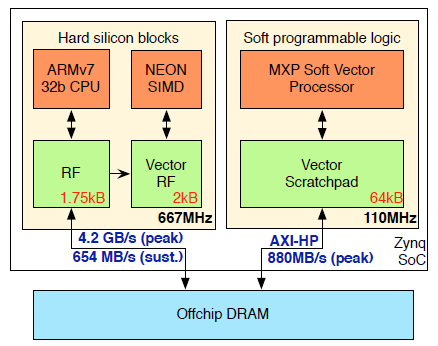
\includegraphics[width=0.67\textwidth]{images/arm-neon-mxp.png}
	\caption{Xilinx Zynq SoC Platform Compute Organization~\cite{kapre2016optimizing}}
	\label{arm-neon-mxp}
\end{figure}


As shown in Figure~\ref{table-arm-neon-mxp}, For byte-level operations, ARMv7 processor is able to provide a peak performance of 0.66 Giga-operations per second (GOPS).
Despite the fact that NEON can perform 8 byte-level operations every clock cycle and able to provide a peak performance of 5.3 GOPS, most compute kernels suffer to take advantage of the performance of NEON engine. 

\begin{figure}
	\centering
	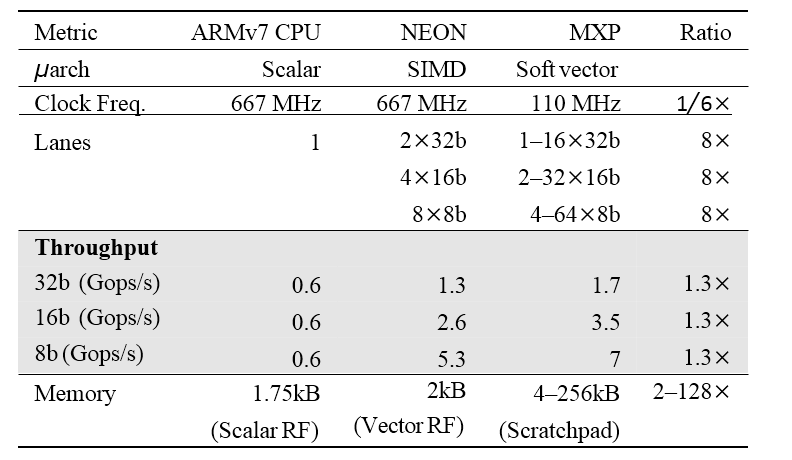
\includegraphics[width=0.67\textwidth]{images/table-arm-neon-mxp.png}
	\caption{Architecture Specifications~\cite{kapre2016optimizing}}
	\label{table-arm-neon-mxp}
\end{figure}



For example, ARMv7 and NEON can provide a performance of only 325 MOPS and 990 MOPS, respectively for quadratic polynomial (as shown in Figure~\ref{quad-poly}). On the other hand, 64-lane MXP soft processor (a carefully designed vector-engine) running at 110 MHz can provide a peak performance of 7 GOPS and while executing quadratic polynomial it can provide a performance of 1.51 GOPS, which is much faster than ARMv7 ($4.75\times$) and NEON ($1.56\times$).





\begin{figure}
	\centering
	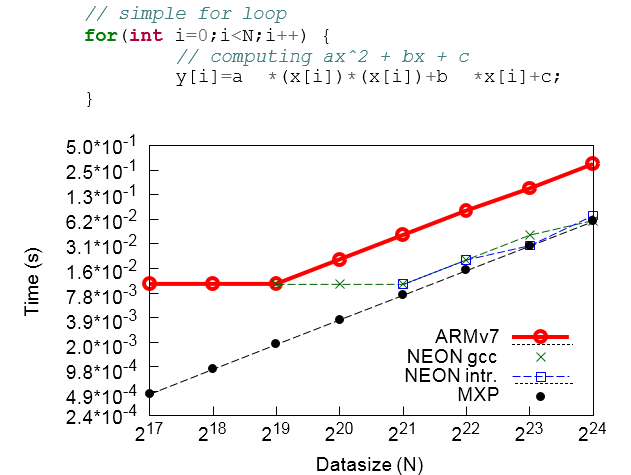
\includegraphics[width=0.9\textwidth]{images/quad-poly.png}
	\caption{Comparing runtime for $a*x^2 + b*x + c$~\cite{kapre2016optimizing}}
	\label{quad-poly}
\end{figure}


In this report, we first analyze compute kernels by extracting data flow graphs and then evaluate the performance of computing platforms such as ARMv7, NEON, Intel processor, and MXP soft vector-engine. The goal is to quatify the gap between peak performance of the platform and achievable performance for a set of compute kernels. 
Major focus of this report is on MXP soft vector-engine which we instantiate on Zynq device available on Zedboard platform.
Apart from using compute kernels to evaluate the performance, we also use a simple image processing application and a complex benchmark (SpMV) to better understand the performance gap.





\section{Contribution}
The main contributions can be summarized as follows:

\begin{itemize}
	\item Setting up Linux and accessing MXP overlay through it so that in future much more attention can be given on building up the MXP application rather than struggling to configure Linux for the MXP overlay.
	\item Comparing the MXP overlay performance against other processors like Intel I3, ARMv7 and NEON hard vector engine for a set of compute kernels.
	\item Accelerating image processing application and a complex benchmark (SpMV) using MXP APIs.
\end{itemize}

\section{Organization}
The remainder of the report is organized as follows:

Chapter 2 gives background information about different computing platforms and most importantly about the MXP vector processor, refer to as an overlay as well. In chapter 3, we describe about the MXP vector processor, it's architecture in detail and the concept of overlapping computation with communication that make it more effective in terms of throughput as compared to other embedded hard vector processors. In chapter 4, we discuss how we configure Linux for MXP on Xilinx ZedBoard so that we can provide OS support for MXP on the Xilinx ZedBoard. In chapter 5, we describe about our experimentation for the performance analysis of MXP vector processor while accelerating compute kernels. In chapter 6, we describe about our experimentation for runtime analysis of image processing application and SpMV computational kernel. We conclude in chapter 7 and discuss future work.








%Field-Programmable Gate Arrays (FPGAs) provides an easier way than Application Specific Integrated Circuits (ASICs) for the implementation of different computing platforms. FPGAs generally yield higher performance and lower power than optimized software running on high-end CPUs. However, designing hardware with FPGAs remains a difficult and time-consuming process. It requires specialized skills and hours-long CAD processing times \cite{1}. The slow place-and-route cycles while accelerating computations using programmable fabric (FPGAs) and non- availability of suitable abstractions prohibits commercial use of such platforms and thus restricting their effective usage to the hardware experts. FPGA virtualization, which is nothing but the use of the overlay architecture such as MXP soft-vector processor, has emerged as an attractive solution by providing fast compilation, run-time management and software-like programmability. These soft processors can extend the capability of embedded hard vector processors because of their improved design productivity and higher-level design abstraction. With the increasing complexity of FPGA platforms, it is being said that the use of overlay architecture will become mainstream \cite{2}. Moreover, the use of Operating system (OS) in a reconfigurable platform helps in managing various hardware tasks, better management of memory and management of the shared resources across the applications. Integrating an overlay architecture with memory subsystem and processor is very important to manage and enable sharing of limited overlay resources. Overlays exhibit features independent from the host FPGA.